% Options for packages loaded elsewhere
\PassOptionsToPackage{unicode}{hyperref}
\PassOptionsToPackage{hyphens}{url}
\PassOptionsToPackage{dvipsnames,svgnames,x11names}{xcolor}
%
\documentclass[
  sn-vancouver,
  Numbered,
  referee,
  lineno]{sn-jnl}



\usepackage{amsmath,amssymb}
\usepackage{iftex}
\ifPDFTeX
  \usepackage[T1]{fontenc}
  \usepackage[utf8]{inputenc}
  \usepackage{textcomp} % provide euro and other symbols
\else % if luatex or xetex
  \usepackage{unicode-math}
  \defaultfontfeatures{Scale=MatchLowercase}
  \defaultfontfeatures[\rmfamily]{Ligatures=TeX,Scale=1}
\fi
\usepackage{lmodern}
\ifPDFTeX\else  
    % xetex/luatex font selection
\fi
% Use upquote if available, for straight quotes in verbatim environments
\IfFileExists{upquote.sty}{\usepackage{upquote}}{}
\IfFileExists{microtype.sty}{% use microtype if available
  \usepackage[]{microtype}
  \UseMicrotypeSet[protrusion]{basicmath} % disable protrusion for tt fonts
}{}
\makeatletter
\@ifundefined{KOMAClassName}{% if non-KOMA class
  \IfFileExists{parskip.sty}{%
    \usepackage{parskip}
  }{% else
    \setlength{\parindent}{0pt}
    \setlength{\parskip}{6pt plus 2pt minus 1pt}}
}{% if KOMA class
  \KOMAoptions{parskip=half}}
\makeatother
\usepackage{xcolor}
\setlength{\emergencystretch}{3em} % prevent overfull lines
\setcounter{secnumdepth}{-\maxdimen} % remove section numbering
% Make \paragraph and \subparagraph free-standing
\makeatletter
\ifx\paragraph\undefined\else
  \let\oldparagraph\paragraph
  \renewcommand{\paragraph}{
    \@ifstar
      \xxxParagraphStar
      \xxxParagraphNoStar
  }
  \newcommand{\xxxParagraphStar}[1]{\oldparagraph*{#1}\mbox{}}
  \newcommand{\xxxParagraphNoStar}[1]{\oldparagraph{#1}\mbox{}}
\fi
\ifx\subparagraph\undefined\else
  \let\oldsubparagraph\subparagraph
  \renewcommand{\subparagraph}{
    \@ifstar
      \xxxSubParagraphStar
      \xxxSubParagraphNoStar
  }
  \newcommand{\xxxSubParagraphStar}[1]{\oldsubparagraph*{#1}\mbox{}}
  \newcommand{\xxxSubParagraphNoStar}[1]{\oldsubparagraph{#1}\mbox{}}
\fi
\makeatother

\usepackage{color}
\usepackage{fancyvrb}
\newcommand{\VerbBar}{|}
\newcommand{\VERB}{\Verb[commandchars=\\\{\}]}
\DefineVerbatimEnvironment{Highlighting}{Verbatim}{commandchars=\\\{\}}
% Add ',fontsize=\small' for more characters per line
\usepackage{framed}
\definecolor{shadecolor}{RGB}{241,243,245}
\newenvironment{Shaded}{\begin{snugshade}}{\end{snugshade}}
\newcommand{\AlertTok}[1]{\textcolor[rgb]{0.68,0.00,0.00}{#1}}
\newcommand{\AnnotationTok}[1]{\textcolor[rgb]{0.37,0.37,0.37}{#1}}
\newcommand{\AttributeTok}[1]{\textcolor[rgb]{0.40,0.45,0.13}{#1}}
\newcommand{\BaseNTok}[1]{\textcolor[rgb]{0.68,0.00,0.00}{#1}}
\newcommand{\BuiltInTok}[1]{\textcolor[rgb]{0.00,0.23,0.31}{#1}}
\newcommand{\CharTok}[1]{\textcolor[rgb]{0.13,0.47,0.30}{#1}}
\newcommand{\CommentTok}[1]{\textcolor[rgb]{0.37,0.37,0.37}{#1}}
\newcommand{\CommentVarTok}[1]{\textcolor[rgb]{0.37,0.37,0.37}{\textit{#1}}}
\newcommand{\ConstantTok}[1]{\textcolor[rgb]{0.56,0.35,0.01}{#1}}
\newcommand{\ControlFlowTok}[1]{\textcolor[rgb]{0.00,0.23,0.31}{\textbf{#1}}}
\newcommand{\DataTypeTok}[1]{\textcolor[rgb]{0.68,0.00,0.00}{#1}}
\newcommand{\DecValTok}[1]{\textcolor[rgb]{0.68,0.00,0.00}{#1}}
\newcommand{\DocumentationTok}[1]{\textcolor[rgb]{0.37,0.37,0.37}{\textit{#1}}}
\newcommand{\ErrorTok}[1]{\textcolor[rgb]{0.68,0.00,0.00}{#1}}
\newcommand{\ExtensionTok}[1]{\textcolor[rgb]{0.00,0.23,0.31}{#1}}
\newcommand{\FloatTok}[1]{\textcolor[rgb]{0.68,0.00,0.00}{#1}}
\newcommand{\FunctionTok}[1]{\textcolor[rgb]{0.28,0.35,0.67}{#1}}
\newcommand{\ImportTok}[1]{\textcolor[rgb]{0.00,0.46,0.62}{#1}}
\newcommand{\InformationTok}[1]{\textcolor[rgb]{0.37,0.37,0.37}{#1}}
\newcommand{\KeywordTok}[1]{\textcolor[rgb]{0.00,0.23,0.31}{\textbf{#1}}}
\newcommand{\NormalTok}[1]{\textcolor[rgb]{0.00,0.23,0.31}{#1}}
\newcommand{\OperatorTok}[1]{\textcolor[rgb]{0.37,0.37,0.37}{#1}}
\newcommand{\OtherTok}[1]{\textcolor[rgb]{0.00,0.23,0.31}{#1}}
\newcommand{\PreprocessorTok}[1]{\textcolor[rgb]{0.68,0.00,0.00}{#1}}
\newcommand{\RegionMarkerTok}[1]{\textcolor[rgb]{0.00,0.23,0.31}{#1}}
\newcommand{\SpecialCharTok}[1]{\textcolor[rgb]{0.37,0.37,0.37}{#1}}
\newcommand{\SpecialStringTok}[1]{\textcolor[rgb]{0.13,0.47,0.30}{#1}}
\newcommand{\StringTok}[1]{\textcolor[rgb]{0.13,0.47,0.30}{#1}}
\newcommand{\VariableTok}[1]{\textcolor[rgb]{0.07,0.07,0.07}{#1}}
\newcommand{\VerbatimStringTok}[1]{\textcolor[rgb]{0.13,0.47,0.30}{#1}}
\newcommand{\WarningTok}[1]{\textcolor[rgb]{0.37,0.37,0.37}{\textit{#1}}}

\providecommand{\tightlist}{%
  \setlength{\itemsep}{0pt}\setlength{\parskip}{0pt}}\usepackage{longtable,booktabs,array}
\usepackage{calc} % for calculating minipage widths
% Correct order of tables after \paragraph or \subparagraph
\usepackage{etoolbox}
\makeatletter
\patchcmd\longtable{\par}{\if@noskipsec\mbox{}\fi\par}{}{}
\makeatother
% Allow footnotes in longtable head/foot
\IfFileExists{footnotehyper.sty}{\usepackage{footnotehyper}}{\usepackage{footnote}}
\makesavenoteenv{longtable}
\usepackage{graphicx}
\makeatletter
\def\maxwidth{\ifdim\Gin@nat@width>\linewidth\linewidth\else\Gin@nat@width\fi}
\def\maxheight{\ifdim\Gin@nat@height>\textheight\textheight\else\Gin@nat@height\fi}
\makeatother
% Scale images if necessary, so that they will not overflow the page
% margins by default, and it is still possible to overwrite the defaults
% using explicit options in \includegraphics[width, height, ...]{}
\setkeys{Gin}{width=\maxwidth,height=\maxheight,keepaspectratio}
% Set default figure placement to htbp
\makeatletter
\def\fps@figure{htbp}
\makeatother

%%%% Standard Packages

\usepackage{graphicx}%
\usepackage{multirow}%
\usepackage{amsmath,amssymb,amsfonts}%
\usepackage{amsthm}%
\usepackage{mathrsfs}%
\usepackage[title]{appendix}%
\usepackage{xcolor}%
\usepackage{textcomp}%
\usepackage{manyfoot}%
\usepackage{booktabs}%
\usepackage{algorithm}%
\usepackage{algorithmicx}%
\usepackage{algpseudocode}%
\usepackage{listings}%

%%%%

\raggedbottom
\makeatletter
\@ifpackageloaded{caption}{}{\usepackage{caption}}
\AtBeginDocument{%
\ifdefined\contentsname
  \renewcommand*\contentsname{Table of contents}
\else
  \newcommand\contentsname{Table of contents}
\fi
\ifdefined\listfigurename
  \renewcommand*\listfigurename{List of Figures}
\else
  \newcommand\listfigurename{List of Figures}
\fi
\ifdefined\listtablename
  \renewcommand*\listtablename{List of Tables}
\else
  \newcommand\listtablename{List of Tables}
\fi
\ifdefined\figurename
  \renewcommand*\figurename{\textbf{Figure}}
\else
  \newcommand\figurename{\textbf{Figure}}
\fi
\ifdefined\tablename
  \renewcommand*\tablename{\textbf{Table}}
\else
  \newcommand\tablename{\textbf{Table}}
\fi
}
\@ifpackageloaded{float}{}{\usepackage{float}}
\floatstyle{ruled}
\@ifundefined{c@chapter}{\newfloat{codelisting}{h}{lop}}{\newfloat{codelisting}{h}{lop}[chapter]}
\floatname{codelisting}{Listing}
\newcommand*\listoflistings{\listof{codelisting}{List of Listings}}
\captionsetup{labelsep=period}
\makeatother
\makeatletter
\makeatother
\makeatletter
\@ifpackageloaded{caption}{}{\usepackage{caption}}
\@ifpackageloaded{subcaption}{}{\usepackage{subcaption}}
\makeatother
\ifLuaTeX
  \usepackage{selnolig}  % disable illegal ligatures
\fi
\usepackage{bookmark}

\IfFileExists{xurl.sty}{\usepackage{xurl}}{} % add URL line breaks if available
\urlstyle{same} % disable monospaced font for URLs
\hypersetup{
  pdftitle={Brain Dynamics},
  colorlinks=true,
  linkcolor={blue},
  filecolor={Maroon},
  citecolor={Blue},
  urlcolor={Blue},
  pdfcreator={LaTeX via pandoc}}

\title[Brain Dynamics]{Brain Dynamics}

% author setup
\author*[1,2]{\fnm{Alexander Mark} \sur{Weber}}\email{aweber@bcchr.ca}
% affil setup
\affil[1]{\orgdiv{BC Children's Hospital Research
Institute}, \orgname{The University of British
Columbia}, \orgaddress{\street{938 West 28th
Avenue}, \city{Vancouver}, \postcode{V5Z 4H4}, \country{Canada}}}
\affil[2]{\orgdiv{Pediatrics}, \orgname{The University of British
Columbia}, \orgaddress{\street{2329 West
Mall}, \city{Vancouver}, \postcode{V6T 1Z4}, \country{Canada}}}

% abstract 

\abstract{An introduction to the idea of brain dynamics in fMRI studies}

% keywords

\begin{document}
\maketitle

\textsuperscript{1} The University of British Columbia\\
\textsuperscript{2} The University of British Columbia

\textsuperscript{*} Correspondence:
\href{mailto:aweber@bcchr.ca}{Alexander Mark Weber
\textless{}aweber@bcchr.ca\textgreater{}}

\section{Introduction}\label{introduction}

Like many physiological data, neurological signals --- such as fMRI-BOLD
--- appear as irregular time-series. Often thought of as being random or
noisy, there was an initial tendency to measure them statistically, such
as calculating their standard deviation, assuming that the elements of
the series were independent. However, this approach is inadequate when
events exhibit interdependence, whether through short- or long-range
temporal correlations (LRTCs) \citep{ekePhysiologicalTimeSeries2000}.
Therefore, there is a need for methods that can both identify and
characterize random noise from irregular but structured and correlated
noise. One such method used for LRTCs is the fractal method.

A fractal structure, either spatial or temporal, is composed of smaller
parts that exhibit the same pattern at every scale
\citep{koch1904, kochMethodeGeometriqueElementaire1906, mandelbrotHowLongCoast1967}.
Classic spatial examples of fractals in nature are coastlines
\citep{mandelbrotHowLongCoast1967}, circulatory system
\citep{jayalalithaFractalModelBlood2008}, and brain anatomy
\citep{ansellUnveilingUniversalAspects2024}, where at each level of
magnification these structures look the same;
i.e.~\emph{self-similarity}. For a dynamic process, or in the temporal
domain, this is known as \emph{scale invariance}, meaning that both
rapid and slow processes follow the same pattern
\citep{rileyTutorialIntroductionAdaptive2012}. These scale-free LRTCs
exhibit a gradual decay in their autocorrelation function, indicating
that the system maintains a long-lasting, multiscale memory of its past
states, which play a role in shaping its present behaviour. Scale-free
behavior is a signature characteristic of complex systems that can be
understood as the collective outcome of numerous interacting components
with weak and random connections
\citep{csermelyWeakLinksStabilizers2006}. Physiological systems, such as
the brain, require a mix of randomness and structure to function
optimally \citep{bakSelforganizedCriticalityExplanation1987}. In many
cases, this balance between order and randomness allows the system to
remain adaptable and responsive to changing conditions
\citep{lipsitzLossComplexityAging1992, lipsitzDynamicsStabilityPhysiologic2002}.
This adaptability is particularly evident when a system is operating
near what is called a `critical point', the phase change between order
and disorder. When a system is operating near the critical point, it is
expected to exhibit LRTCs. Therefore, by analyzing the LRTC of a
time-series, valuable insights can be found into the underlying
mechanisms driving system behavior, such as memory effects,
self-organization, and criticality \citep{beggsCortexCriticalPoint2022}.

\begin{center}\rule{0.5\linewidth}{0.5pt}\end{center}

\begin{quote}
``Because pink noise lies between white and Brown(ian) noise, it has
been proven to bring stability and adaptability into dynamic processes,
thus, crucial properties of well-functioning complex systems''
\citep{bakSelforganizedCriticalityExplanation1987}
\end{quote}

\begin{quote}
``as pink noise arises from the interaction of multiple systems and
operates over different scales, it has been shown to contribute to
system resiliency and structural integrity if individual components were
lost or interrupted''
\citep{lipsitzLossComplexityAging1992, lipsitzDynamicsStabilityPhysiologic2002}
\end{quote}

See \citet{hermanFractalCharacterizationComplexity2009} for a really
good review

Another good review is by Werner (2010) linking fractals/Hurst and
Criticality \citet{wernerFractalsNervousSystem2010}

\begin{quote}
``This 1/f power relationship implies that perturbations occurring at
slow frequencies can cause a cascade of energy dissipation at higher
frequencies so that widespread slow oscillations, observed with BOLD
contrast fMRI, are modulating faster local events {[}12{]}.'' from
\citet{barnesEndogenousHumanBrain2009}
\end{quote}

\begin{quote}
``Systems operating at a phase transition are metastable with respect to
a set of control parameters, and capable of rapid qualitative change in
response to external stimuli.'' Moreover, these transitions occur over
short and long spatial and temporal scales (Freeman, 2003) lending
credence to the proposition that the brain is maintained in a state of
self-organised criticality (Bak et al, 1987). Whilst these models are
incomplete in their description of the cortex, they draw interesting
parallels with the scale-invariant, small-world topologies observed from
resting state fMRI and MEG data (Achard et al, 2006; Achard et al,
2008). From these observations and the results presented in this study,
self-organised criticality appears to offer a tractable association
between the spatial and temporal behaviours of the brain. from
\citet{sucklingEndogenousMultifractalBrain2008}
\end{quote}

\begin{center}\rule{0.5\linewidth}{0.5pt}\end{center}

\section{Fractal Dimension and Hurst
Exponent}\label{fractal-dimension-and-hurst-exponent}

Non-periodic fluctuations are prevalent in physiological systems, and
these irregular patterns can be mathematically modeled using stochastic,
chaotic, or noisy chaotic methods. Stochastic models assume that the
fluctuations result from a large number of weak influences, while
chaotic models conceptualize that strong nonlinear interactions between
a few factors shape the fluctuations. Among the various stochastic
approaches, `fractal' models offer the most accurate representation of
reality by considering the self-similar nature of physiological
fluctuations over different time scales
\citep{ekeFractalCharacterizationComplexity2002}. Fractal structures
were first expressed in the late 19th and early 20th century by
mathematicians who generated complex geometrical structures with simple
objects (e.g.~a triangle) by applying a simple rule of transformation in
an infinite number of iterative steps Figure~\ref{fig-fractal}. A
use-case for these geometric structures was not fully realized until the
1960s, when Benoit Mandelbrot formalized them as a new form of geometry
capable of describing the complex shapes and forms of nature
\citep{mandelbrotHowLongCoast1967}.

\begin{figure}[H]

\centering{

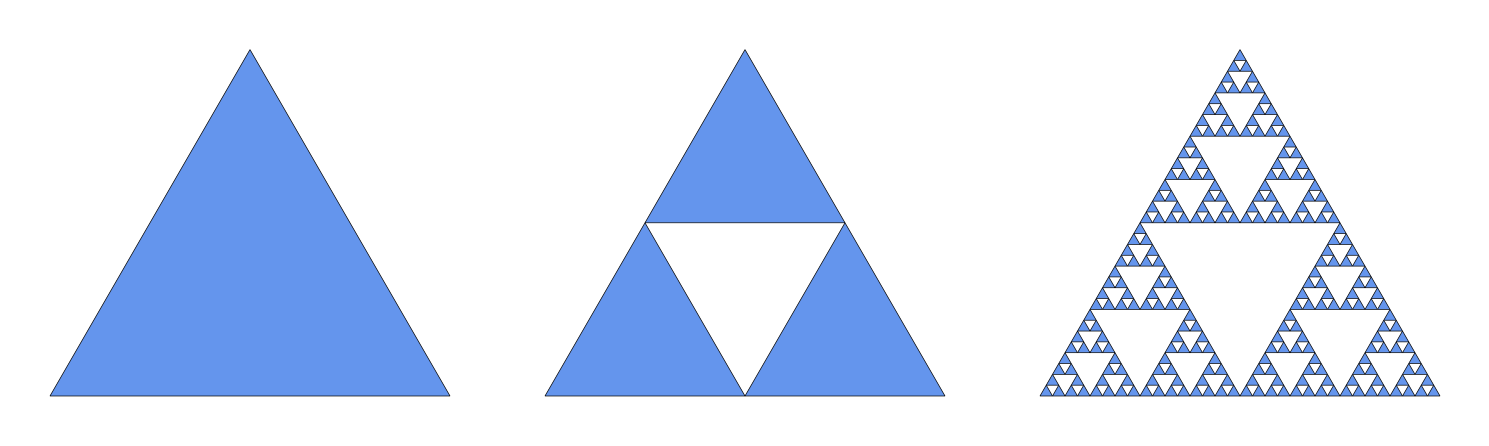
\includegraphics{index_files/figure-latex/notebooks-Figures-fig-fractal-output-1.png}

}

\caption{\label{fig-fractal}\textbf{Ideal mathematical fractal.} The 2D
Sierpinski triangle starts with a simple equilateral triangle (left),
and subdivides it recursively into smaller equilateral triangles. For
every iteration, each triangle (in blue) is further subdivided it into
four smaller congruent equilateral triangles with the central triangle
removed. The first such iteration is shown in the centre, with the fifth
iteration shown on the right.}

\end{figure}%

\textsubscript{Source:
\href{https://WeberLab.github.io/Hurst_LitReview/notebooks/Figures-preview.html\#cell-fig-fractal}{Figures}}

Unlike Euclidean structures that can use axioms and rules to describe an
object of integer dimensions, fractal structures can only be
characterized by recursive algorithms that extend the use of dimension
to the non-integer range \citep{hermanFractalBranchingPattern2001}.
Recognizing this difference, Mandelbrot named these complex structures
`fractals', and defined their non-Euclidean dimension as a `fractal
dimension' (FD) --- that is, a non-integer. For the one-dimensional
time-series, FD will be between 1 and 2. While a structure such as the
Sierpinski triangle is an `exact fractal', meaning it is assembled from
pieces that are an exact replica of the whole, nature is composed of
`statistical fractals', whose self-similarity is found in the power law
scaling of the parameters characterizing their structures at different
scales of observation Figure~\ref{fig-statisticalfractal}. Unlike
Euclidean structures which can be defined by axioms, fractals can only
be characterized by a set of properties that, when present, indicate the
structure is indeed fractal (see Section~\ref{sec-properties}).

\begin{figure}

\centering{

\includegraphics{./image/exact_vs_statistical_tree.png}

}

\caption{\label{fig-statisticalfractal}\textbf{A comparison of
statistical and exact fractal patterns.} The two basic forms of fractals
are demonstrated. Zooming in on tree branches (left), an exact
self-similar element cannot be found. Zooming in on an exact fractal
(right), exact replica of the whole are found. Photo by author.
Branching fractal made in Python. Figure inspired by Taylor (2006)
\citep{taylorPersonalReflectionsJackson2006}}

\end{figure}%

The Hurst exponent (H) is a statistical measure used to quantify
long-range dependence or persistence in time-series data (i.e.~LRTCs).
First introduced by Harold Hurst in 1951 for hydrological applications
\citep{hurstLongTermStorageCapacity1951}, it was Mandelbrot again who
helped popularize its use for studying complex shapes and forms of
nature
\citep{mandelbrotClasseProcessusStochastiques1965, mandelbrotHowLongCoast1967}.
Since then it has been applied across various fields, including finance,
geophysics, ecology, and neuroscience, to characterize complex systems
with intricate dynamics
\citep{molzFractionalBrownianMotion1997, korvinFractalModelsEarth1992, parkSelfSimilarNetworkTraffic2000, gravesBriefHistoryLong2017}.
H and FD for time-series can be directly converted, as
\begin{equation}\phantomsection\label{eq-HRD}{
H=2–D.
}\end{equation} This means that FD and H are inversely correlated, and
that H is a real number between 0 and 1 (non-inclusive; although it can
be extended to \textgreater{} 1; see \ldots). For the rest of this
paper, we will be discussing H.

\emph{Thus, the basic premise behind fractal time-series analysis is:
beneath the seemingly chaotic and unpredictable variations in the
signal, there lies a stable underlying mechanism which can be
effectively described using only a few possible parameters (i.e.~H or
FD).}

\subsection{Properties}\label{sec-properties}

When H = 0.5 (FD = 1.5), the time-series is completely uncorrelated, has
no memory, and is like white noise (pure random). It represents the
highest level of unpredictability and entropy, but not necessarily the
most complex state in a physiological sense. When H \textless{} 0.5 (FD
\textgreater{} 1.5), the time-series is said to be anti-persistent,
exhibiting negative correlations: i.e.~if the signal increases at one
point, it's likely to decrease at the next point. This is also known as
short-term reversal. This tends to make the time-series more predictable
and reduces randomness, often simplifying dynamics. When H
\textgreater{} 0.5 (FD \textless{} 1.5), the time-series exhibits
positive long-range correlations, and is more structured. The
time-series displays a long-term trend, meaning past states influence
future states.

There are four main properties that must be present for a time-series to
be characterized by H or FD: 1) self-similarity; 2) power law scaling
relationship; 3) scale-invariance; and 4) a scaling range
(Figure~\ref{fig-fourprop}). Each of these will be discussed in turn.

\subsubsection{Self-similarity}\label{self-similarity}

Self-similarity means that pieces of the structure, when enlarged,
resemble larger pieces or the whole (Figure~\ref{fig-statisticalfractal}
and Figure~\ref{fig-fourprop} A-C). Technically speaking, physiological
time-series are self-affine, meaning their scaling is anisotropic
(i.e.~the proportions between enlarged pieces are different in one
direction from those in the other). This is because in one direction
(time) the proportions between the enlarged pieces is different than in
the other (amplitude of signal; e.g.~fMRI BOLD)
\citep{ekePhysiologicalTimeSeries2000}.

\subsubsection{Power law scaling
relationship}\label{power-law-scaling-relationship}

Power law scaling means that, for a quantitative property, \(q\), is
measured in quantities of \(s\), its value depends on \(s\) according to
the following scaling relationship:

\begin{equation}\phantomsection\label{eq-qfs}{
q=f(s).
}\end{equation}

For non-fractal objects, the estimate of \(q\) using progressively
smaller units of measure \(s\) will converge to a single value as the
size of the measurement units approaches zero. On the other hand,
fractals exhibit a power law scaling relationship with \(s\), whereby
the estimated value of \(q\) increases without limit as the size of the
\(s\) decreases.

\begin{equation}\phantomsection\label{eq-powerlawscalingrelationship}{
q=ps^{\epsilon}
}\end{equation}

where \(p\) is a factor of proportionality (prefactor) and \(\epsilon\)
is a negative number, the scaling exponent. The value of \(\epsilon\)
can be determined as the slope of the linear regression fit to the data
pairs on the plot of \(\log{q}\) versus \(\log{s}\):

\begin{equation}\phantomsection\label{eq-logpowerlawscaling}{
\log{q} = \log{p} + \epsilon\log{s}
}\end{equation}

Data points for exact fractals will line up along perfectly with a
linear-regression slope, while statistical fractals will scatter around
it since the two sides of Equation~\ref{eq-logpowerlawscaling} are equal
only in distribution.

\subsubsection{Scale-invariance}\label{scale-invariance}

The ratio of two estimates of \(q\) measured at two different scales,
\(s_{1}\) and \(s_{2}\), \(q_{2}/q_{1}\) depends only on the ratio of
scales (relative scale), \(s_{2}/s_{1}\), and not directly on the
absolute scale, \(s_{1}\) or \(s_{2}\)

\begin{equation}\phantomsection\label{eq-scaleinv}{
q_{2}/q_{1} = ps_2^\epsilon / ps_1^\epsilon = (s_2 / s_1)^\epsilon
}\end{equation}

For statistical fractals, like those of nature, \(s_2/s_1\) may change
in a continuous fashion still leaving the validity of
Equation~\ref{eq-scaleinv} unaffected. The scale-invariance of fractals
arises from the fact that the geometrical structure only depends on the
scaling factor (ratio of scales), and not the absolute scale. As a
result, quantitative properties of smaller parts are similar to those of
larger parts.

\subsubsection{Scaling range}\label{scaling-range}

Natural fractals may only display scale-invariance within a restricted
range, as they are finite (either by definition or due to the fact that
they must be sampled). The upper cut-off point (\(s_{max}\)) in
Equation~\ref{eq-scalerange}, falls within the size range of the
structure itself. Similarly, the lower cut-off point (\(s_{min}\)) falls
within the dimensions of the smallest structural elements. The scaling
range (SR) is defined in decades

\begin{equation}\phantomsection\label{eq-scalerange}{
\text{SR} = \log_{10}(s_{max}/s_{min})
}\end{equation}

\begin{figure}[H]

\centering{

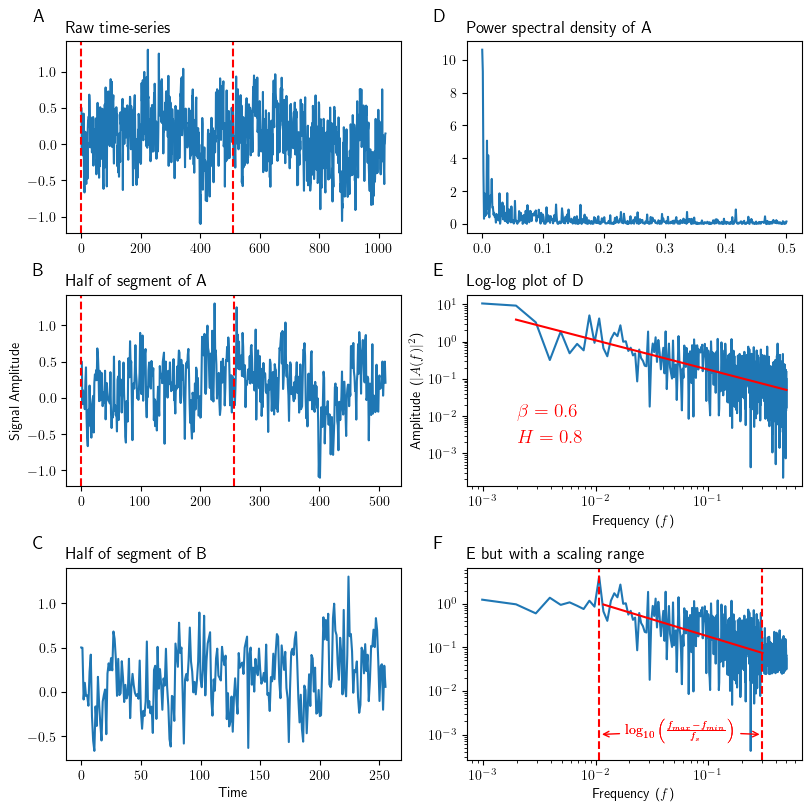
\includegraphics{index_files/figure-latex/notebooks-Figures-fig-fourprop-output-1.png}

}

\caption{\label{fig-fourprop}\textbf{Main properties of a fractal
time-series} A-C show a raw time-series (fractional Gaussian noise in
this example) at different scales: B is the first half of A (shown as
vertical dashed lines in A), while C is half of B (shown in vertical
dashed lines in B). D is a power spectral density plot of A. E shows D
but on a log-log plot, demonstrating the linear nature of fractal
signals when plotted on a log-log scale. The slope of E is \(-\beta\).
In this example, \(\beta\) is calculated to be 0.6, which translates to
an H of 0.8. F shows a modified version of E, which imagines that E only
demonstrates a power law scaling relationship between two distinct
frequencies. The equation for calculating the scaling range in decades
is shown. Exact fractal time-series (A) was created using the
Davies-Harte method.}

\end{figure}%

\textsubscript{Source:
\href{https://WeberLab.github.io/Hurst_LitReview/notebooks/Figures-preview.html\#cell-fig-fourprop}{Figures}}

\subsection{Prerequisites to measuring
H}\label{prerequisites-to-measuring-h}

\subsubsection{Time-points}\label{time-points}

Before determining if a time-series exhibits a power-law scaling
relationship, one should first determine if the time-series has enough
time-points to do so. The rule of thumb is that the power law
relationship should be present in a range larger than two decades in the
frequency domain of a PSD \citep{ekePhysiologicalTimeSeries2000}. Due to
the Whittaker--Nyquist-Shannon sampling theorem
\citep{shannonCommunicationPresenceNoise1949}, one requires two times as
many time-points as frequency samples. Since two decades in the
frequency domain is 100 distinct frequencies, one would required at
least 200 fMRI volumes / time-points to proceed (not including
non-steady state volumes). Furthermore, many algorithms for measuring H
require powers of 2, bringing the recommended number of volumes to 256.
With a TR of 1s, this translates to \(\sim\) 5 minutes (and 10 minutes
for the more common TR of 2s).

\subsubsection{Power-law scaling
relationship}\label{power-law-scaling-relationship-1}

The next step would be to perform a periodogram or PSD and test for a
power-law scaling relationship. Usually power laws are tested using a
probability distribution
\citep{clausetPowerLawDistributionsEmpirical2009}. However, as the PSD
is not a probability distribution, alternative methods must be used. A
goodness-of-fit test can be devised based on
\citet{clausetPowerLawDistributionsEmpirical2009}, which can also help
us derive the SR (i.e.~\(freq_{min}\) and \(freq_{max}\)). First, a PSD
is produced, and the variance (\(\sigma^2\)), \(\beta\), and H are
computed using Equation~\ref{eq-psdH}. Next, the Kolmogorov--Smirnov
(KS) statistic
\citep{kolmogorovSullaDeterminazioneEmpirica1933, smirnovTableEstimatingGoodness1948}
is used to measure the distance D between the raw PSD data-points and
the best-fit linear-regression line used to calculate H (i.e.~the
residuals). The D in this case is the largest residual error. Then,
1,000 time series of either fGn or fBm (depending on what value of
\(\beta\) was found; see Equation~\ref{eq-psdH}) with the same length,
\(\sigma^2\), and Hurst exponent are generated using a simulated exact
fractal signal (spectral synthesis method (SSM)
\citep{peitgenScienceFractalImages1988}, Davies-Harte method (DH)
\citep{daviesTestsHurstEffect1987}, Cholesky method
\citep{asmussenStochasticSimulationView1998}, the Hosking's method
\citep{hoskingModelingPersistenceHydrological1984} or the ARFIMA
simulation method
\citep{roumeBiasesSimulationAnalysis2019, grangerINTRODUCTIONLONGMEMORYTIME1980}).
The 1,000 synthetic time-series are then converted to PSDs, and the KS
distance is again measured. The \(p\)-value is defined as the fraction
of synthetic time series with Ds that are larger than the D of the
original time-series. The larger the \(p\)-value, the more plausible the
synthetic model (either fGn or fBm) is for representing the original
time-series, and the better the fit of the original data to a scale-free
distribution. The null-hypothesis that the time-series is not scale free
is rejected if \(p\) \textless{} 0.05 (i.e.~if \(p\) \textgreater{}
0.05, we say that the time-series is scale-free).

It is important to note, however, that the \(p\)-value in question may
need to be adjusted based on the number of time-points.

A sample python code is provide in Section~\ref{sec-powerlawscalingcode}

\subsubsection{Scaling range}\label{scaling-range-1}

As previously mentioned, statistical fractals are unlikely to display
their power-law scaling relationship across all scales. Therefore, it is
important to test the scaling relationship across a range of scales,
determining the minimum and maximum scale for which the scaling
relationship exists (if at all). One way to determine this range is to
apply the power-law scaling test across a range of scales, starting with
the full range, and progressively reducing the size while trying to
maintain the widest range.

However, this method can be computationally intensive, and prone to
false negatives, especially signals with very high or low H values. One
solution is, instead of applying this test to every voxel in a 4D fMRI
brain scan, to segment the brain into separate ROIs (e.g.~anatomically
based on an atlas, or functionally by first running ICA to identify
RSNs), average the time-series within each ROI, which will improve SNR,
and then run the power-law scaling test.

Once a scaling range is discovered, it is then important to use this
range when measuring H. For example, if H is being calculated using a
frequency approach, the linear regression can be limited to within the
frequency range. However, if another approach is used, a bandpass filter
may be necessary first to remove unwanted frequencies. Careful attention
should be paid to the type of frequency filtering method employed, and
care must be taken not to re-introduce nuissance regressors previously
removed \citep{lindquistModularPreprocessingPipelines2019}.

\subsection{Classification: Gaussian noise vs Brownian
motion}\label{classification-gaussian-noise-vs-brownian-motion}

If the prerequisites above have been met, the next step is to classify
the signal type. Fractal signals can be organized into two distinct
kinds: fractional Gaussian noise (fGn) and fractional Brownian motion
(fBm) Figure~\ref{fig-typicalsamplepaths}. fGn signals are stationary,
meaning they tend to center along a mean and variance value over time.
In contrast, fBm signals are non-stationary: their values tend to wander
away from the mean, and their variance is a power function of the time
span over which it is computed. Curiously, fGn and fBm can easily be
converted from one to the other: fGn to fBm by applying a successive
summation between elements of the fGn series; and fBm to fGn by applying
successive differences between elements of a fBm series.

When calculating the H of a signal, it is imperative to first classify
the signal as either fGn or fBm. Failure to do so can result in serious
miscalculation of H, as different estimators can produce extremely
biased calculations depending on the assumed type of signal. The
distinction between fGn and fBm can be seen in their spectral
properties. Applying a Fourier transform of a signal to convert it from
the time-domain to the frequency domain, we can obtain a power spectral
density, which relates the amplitude of the frequency (y-axis) to the
frequency (x-axis). The PSD of fGn signals follow a power-law form:
\(|A(f)|^2 \propto f^{-\beta}\), where the exponent \(\beta\) ranges
between -1 and 1. This is known as \(1/f\) noise, as the power is
inversely proportional to frequency. fBm, being a cumulative sum of fGn,
has a different spectral behaviour:
\(|A(f)|^2 \propto f^{-(\beta + 2)}\). This steeper decay
(\(\beta + 2\)) causes fBm to exhibit stronger low-frequency dominance,
making it distinct from \(1/f\) noise. Thus, when \(\beta \sim 1\), a
signal is said to exist on the \(1/f\) boundary.

One method of calculating H, known as the spectral method or periodogram
method (PM), is based on the PSD. The PM method involves creating a
log-log plot of the time-series' periodogram using a fast Fourier
transform (FFT; Figure~\ref{fig-fourprop} D and E), calculating the
linear-regression slope (\(-\beta\)), and, depending on the slope angle,
using one of two equations:

\begin{equation}\phantomsection\label{eq-psdH}{
H =
\begin{cases}
\frac{\beta + 1}{2}, & \text{if } -1 < \beta < 1 \\
\frac{\beta - 1}{2}, & \text{if } 1 < \beta < 3
\end{cases}
}\end{equation}

\begin{figure}[H]

\centering{

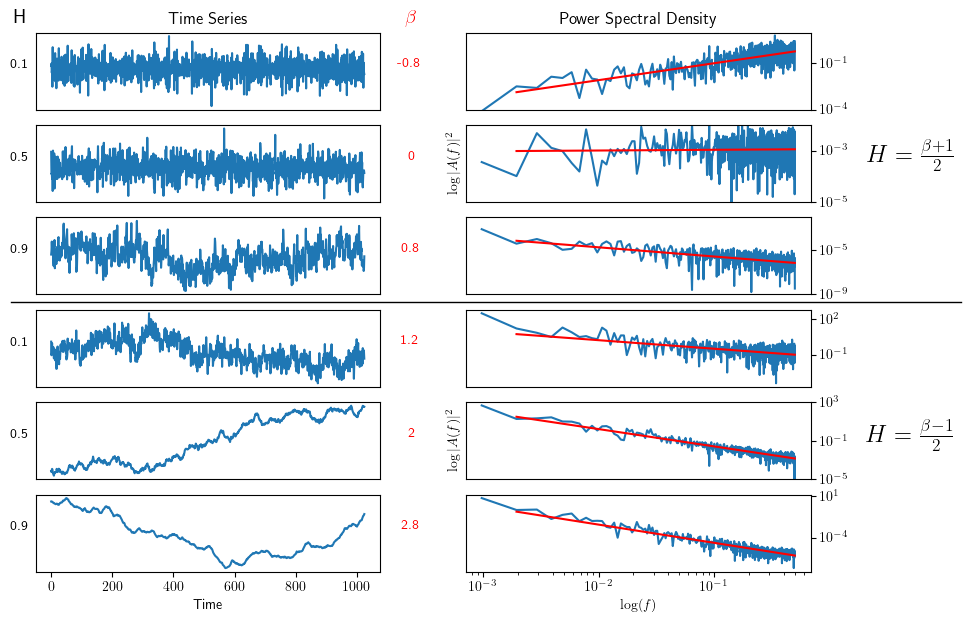
\includegraphics{index_files/figure-latex/notebooks-Figures-fig-typicalsamplepaths-output-1.png}

}

\caption{\label{fig-typicalsamplepaths}\textbf{Simulated fractional
Gaussian noise and fractional Brownian motion.} Raw simulated
time-series with 1,024 time-points and known Hurst values are plotted on
the left. The top three time-series are fractional Gaussian noise, while
the bottom three are fractional Brownian motion. H values are displayed
on the left, while \(\beta\) values are displayed on the right. Note how
fractional Gaussian noise remain centered around a mean
(i.e.~stationary), while fractional Brownian motion wanders away from
the mean (i.e.~non-stationary). Log-log power spectral density plots of
the signals on the left are shown on the right. Linear-regression fits
are shown in red, which are used to calculate \(\beta\) and H using the
appropriate equation (on the right). Exact fractal time-series were
created using the Davies-Harte method.}

\end{figure}%

\textsubscript{Source:
\href{https://WeberLab.github.io/Hurst_LitReview/notebooks/Figures-preview.html\#cell-fig-typicalsamplepaths}{Figures}}

If the class of signal is not appropriately identified --- for example,
when \(\beta\) is \(\sim\) 1 --- it is possible for a true H \(\sim\)
0.9 to be calculated as 0.1. Therefore, algorithms and research in
properly classifying fractal signals is crucially important.

Several methods have been proposed for classifying fGn and fBm signals,
including ones that make use of the PM described above
\citep{ekePhysiologicalTimeSeries2000, ekeFractalCharacterizationComplexity2002},
detrended fluctuation analysis (DFA)
\citep{pengLongrangeAnticorrelationsNonGaussian1993}, autoregressive
fractionally integrated moving average (ARFIMA)
\citep{grangerINTRODUCTIONLONGMEMORYTIME1980}, and wavelet entropy
\citep{ramirezpachecoDistinguishingStationaryNonstationary2012, ramirez-pachecoClassificationFractalSignals2017}.
These methods, however, all struggle to distinguish signals whose PSD
\(\beta\) values are \(\sim\) 1 \citep{ekePhysiologicalTimeSeries2000}
(AKA the \(1/f\) boundary).

\subsubsection{fMRI Signals}\label{fmri-signals}

Are fMRI signals expected to be fGn or fBm?

\subsection{Measuring H}\label{measuring-h}

Fractal analysis tools vary in performance, assumptions, and
limitations. In order to avoid biasing ones results
{[}\citet{bassingthwaighteEvaluatingRescaledRange1994}; @; @; @{]}, it
is important to choose the right method carefully, especially when
applied to physiological signals which can be contaminated by unrelated
noise. The following is a non-exhaustive list of methods, and their
relative strengths and weaknesses. Despite their diversity, all
approaches employ a version of scale-invariance analysis, by fitting a
log feature versus log scale for finding a scaling exponent from a
regression slope, and then calculating H from this scaling exponent.
These methods, however, can be subdivided into those that

\begin{itemize}
\tightlist
\item
  ARIMA (autoregressive integrated moving average) and ARFIMA
  (autoregressive fractionally integrated moving- average)
\item
  Adaptive fractal analysis
  (https://www.frontiersin.org/journals/physiology/articles/10.3389/fphys.2020.00827/full)
\end{itemize}

\subsubsection{Time-domain}\label{time-domain}

\paragraph{Rescaled range analysis
(R/S)}\label{rescaled-range-analysis-rs}

This is the original method used by Hurst in 1951 when studying
hydrology and the long term storage capacity of dams
\citep{hurstLongTermStorageCapacity1951}.

\citet{dongHurstExponentAnalysis2018}

\paragraph{Dispersional analysis (DA)}\label{dispersional-analysis-da}

\citep{bassingthwaightePhysiologicalHeterogeneityFractals1988}

\citet{donaTemporalFractalAnalysis2017}
\citet{donaFractalAnalysisBrain2017}

\paragraph{Scaled window variance
(SWV)}\label{scaled-window-variance-swv}

\citet{donaTemporalFractalAnalysis2017}
\citet{donaFractalAnalysisBrain2017}

\paragraph{Generalized Hurst exponent
(GHE)}\label{generalized-hurst-exponent-ghe}

\paragraph{Triangle total areas (TTA)}\label{triangle-total-areas-tta}

\paragraph{Higuchi method (HM)}\label{higuchi-method-hm}

\paragraph{Central estimation (AM \&
AV)}\label{central-estimation-am-av}

\paragraph{Detrended fluctuation analysis
(DFA)}\label{detrended-fluctuation-analysis-dfa}

\paragraph{Least squares method via standard deviation
(LSSD)}\label{least-squares-method-via-standard-deviation-lssd}

Bayesian

\paragraph{Least squares method via variance
(LSV)}\label{least-squares-method-via-variance-lsv}

\paragraph{Whittle's estimator (WE)}\label{whittles-estimator-we}

\subsubsection{Frequency-domain}\label{frequency-domain}

\paragraph{Periodogram method (PM)}\label{periodogram-method-pm}

\paragraph{\texorpdfstring{Welch technique
(PSD\textsubscript{Welch})}{Welch technique (PSDWelch)}}\label{welch-technique-psdwelch}

\paragraph{Local Whittle (LW)}\label{local-whittle-lw}

Bayesian?

\subsubsection{Mixture}\label{mixture}

\paragraph{Average wavelet coefficient (AWC)
https://journals.aps.org/pre/abstract/10.1103/PhysRevE.58.2779}\label{average-wavelet-coefficient-awc-httpsjournals.aps.orgpreabstract10.1103physreve.58.2779}

\paragraph{Variance vs level (VVL)}\label{variance-vs-level-vvl}

\paragraph{Maximum likelihood in the wavelet domain
(MLW)}\label{maximum-likelihood-in-the-wavelet-domain-mlw}

\begin{quote}
Each fractal analysis tool has different performance, prerequisite
conditions, and limitations, and each needs thorough evaluation in order
to avoid bias or misinterpretation of the derived fractal parameters
{[}5, 6, 8, 9{]}, especially when applied to physiological signals which
may be contaminated with noise {[}15, 28{]}. from
\citep{ekePhysiologicalTimeSeries2000}
\end{quote}

\subsection{Neuroscience Applications}\label{neuroscience-applications}

H has emerged as a valuable tool in neuroscience and clinical research.
Typically, H values reported in adult brains are above 0.5, with higher
H values in grey matter than white matter or cerebrospinal fluid
\citep{dongHurstExponentAnalysis2018, winkMonofractalMultifractalDynamics2008}.
Some key findings from neuroscience research include: a decrease in H
during task performance
\citep{ciuciuInterplayFunctionalConnectivity2014, heScaleFreePropertiesFunctional2011};
negative correlations with task novelty and difficulty
\citep{churchillSuppressionScalefreeFMRI2016}; increases with age in the
frontal and parietal lobes \citep{dongHurstExponentAnalysis2018}, and
hippocampus \citep{winkAgeCholinergicEffects2006}; decreases with age in
the insula, and limbic, occipital and temporal lobes
\citep{dongHurstExponentAnalysis2018}; H \textless{} 0.5 in preterm
infants \citep{mellaTemporalComplexityBOLDsignal2024}; and more
\citep{campbellMonofractalAnalysisFunctional2022}. In terms of clinical
findings, abnormal H values have been identified in Alzheimer's disease
(AD)
\citep{maximFractionalGaussianNoise2005, warsiCorrelatingBrainBlood2012},
autism spectrum disorder (ASD)
\citep{donaTemporalFractalAnalysis2017, laiShiftRandomnessBrain2010, linkeAlteredDevelopmentHurst2024, uscatescuUsingExcitationInhibition2022},
mild traumatic brain injury \citep{donaFractalAnalysisBrain2017}, major
depressive disorder
\citep{weiIdentifyingMajorDepressive2013, jingIdentifyingCurrentRemitted2017}
and schizophrenia
\citep{sokunbiNonlinearComplexityAnalysis2014, uscatescuUsingExcitationInhibition2022}.

\subsection{fMRI preprocessing
considerations}\label{fmri-preprocessing-considerations}

\subsubsection{Nuissance regression}\label{nuissance-regression}

When attempting to regress out non-BOLD signal, it is important to apply
the regression at the same time, and not in succession. Even performing
a band-pass filter after nuissance regression can re-introduce noise
components \citep{lindquistModularPreprocessingPipelines2019}.

\subsubsection{Detrending}\label{detrending}

see \citet{tanabeComparisonDetrendingMethods2002}

\section{Hurst Reviews}\label{hurst-reviews}

\subsection{Table}\label{table}

\begin{longtable}[]{@{}
  >{\raggedright\arraybackslash}p{(\columnwidth - 12\tabcolsep) * \real{0.2308}}
  >{\raggedright\arraybackslash}p{(\columnwidth - 12\tabcolsep) * \real{0.0769}}
  >{\raggedright\arraybackslash}p{(\columnwidth - 12\tabcolsep) * \real{0.0769}}
  >{\raggedright\arraybackslash}p{(\columnwidth - 12\tabcolsep) * \real{0.2308}}
  >{\raggedright\arraybackslash}p{(\columnwidth - 12\tabcolsep) * \real{0.2308}}
  >{\raggedright\arraybackslash}p{(\columnwidth - 12\tabcolsep) * \real{0.0769}}
  >{\raggedright\arraybackslash}p{(\columnwidth - 12\tabcolsep) * \real{0.0769}}@{}}
\caption{\textbf{fMRI-Hurst studies.} An attempt to gather all published
fMRI studies that have used Hurst or Hurst-like analysis, some stats,
and the main findings. Main findings are almost certainly more nuanced
than how we have reported them here; we have attempted to condense the
findings as succinctly as possible. n = number of subjects in the study;
TR = repition time; MLWD = maximum likelihood wavelet;
PSD\textsubscript{Welch} = power spectral density Welch method; DMN =
default mode network; DFA = detrended fluctuation analysis; DA =
dispersional analysis; SWV = scaled window variance; RS = rescaled
range; LW = local Whittle;}\label{tbl-fmrihurst}\tabularnewline
\toprule\noalign{}
\begin{minipage}[b]{\linewidth}\raggedright
Study
\end{minipage} & \begin{minipage}[b]{\linewidth}\raggedright
n
\end{minipage} & \begin{minipage}[b]{\linewidth}\raggedright
Age range
\end{minipage} & \begin{minipage}[b]{\linewidth}\raggedright
Methods
\end{minipage} & \begin{minipage}[b]{\linewidth}\raggedright
Volumes
\end{minipage} & \begin{minipage}[b]{\linewidth}\raggedright
TR (s)
\end{minipage} & \begin{minipage}[b]{\linewidth}\raggedright
Results
\end{minipage} \\
\midrule\noalign{}
\endfirsthead
\toprule\noalign{}
\begin{minipage}[b]{\linewidth}\raggedright
Study
\end{minipage} & \begin{minipage}[b]{\linewidth}\raggedright
n
\end{minipage} & \begin{minipage}[b]{\linewidth}\raggedright
Age range
\end{minipage} & \begin{minipage}[b]{\linewidth}\raggedright
Methods
\end{minipage} & \begin{minipage}[b]{\linewidth}\raggedright
Volumes
\end{minipage} & \begin{minipage}[b]{\linewidth}\raggedright
TR (s)
\end{minipage} & \begin{minipage}[b]{\linewidth}\raggedright
Results
\end{minipage} \\
\midrule\noalign{}
\endhead
\bottomrule\noalign{}
\endlastfoot
Akhrif et al.~(2018) \citep{akhrifFractalAnalysisBOLD2018} & 103 & 19-28
& AFA & task: 425, resting: 350 & 2 & impulsivity: \(\downarrow\) \\
Barnes et al.~(2009) \citep{barnesEndogenousHumanBrain2009} & 14 & 21-29
& MLW & 2048 & 1.1 & cognitive effort: \(\downarrow\) H \\
Campbell et al.~(2015) \citep{campbellFractalBasedAnalysisFMRI2022} & 72
& mean 29 & PSD\textsubscript{Welch} & 900 & 1 & movie-watching:
\(\uparrow\) H in visual, somatosensory, and dorsal attention;
\(\downarrow\) frontoparietal and DMN \\
Churchill et al.~(2015) \citep{churchillScalefreeBrainDynamics2015} & 97
(28 chemo; 37 radiation; 32 HC) & n/a & DFA, Wavelet & 285 & 1.5 &
worry: \(\downarrow\) H \\
Churchill et al.~(2016) \citep{churchillSuppressionScalefreeFMRI2016} &
three datasets (98): 19; 49; 30 & 20-82 & DFA, PSD\textsubscript{Welch}
& \(\sim\) 300 & 2 & age, task novelty and difficulty: \(\downarrow\)
H \\
Ciuciu et al.~(2014) \citep{ciuciuInterplayFunctionalConnectivity2014} &
17 & 18-27 & Wavelet & 194 & 2.16 & networks \\
Dona et al.~(2017) \citep{donaTemporalFractalAnalysis2017} & 71 (56 ASD;
15 HC) & mean 13 & PSD, DA, SWV & 300 & 2 & ASD: \(\uparrow\) H \\
Dona et al.~(2017) \citep{donaFractalAnalysisBrain2017} & 110 (55 mTBI;
55 HC) & mean 13 & PSD, DA, SWV & 180 & 2 & mTBI: \(\uparrow\) H \\
Dong et al.~(2018) \citep{dongHurstExponentAnalysis2018} & 116 & 19-85 &
RS & 260 & 2.5 & age: \(\uparrow\) H frontal and parietal lobe;
\(\downarrow\) H insula, limbic, occipital, temporal lobes \\
Drayne et al.~(2024) \citep{drayneLongrangeTemporalCorrelation2024} & 98
& preterm & PSD\textsubscript{Welch} & 100 & 3 & preterm: \(\downarrow\)
H; differentiates networks \\
Erbil et al.~(2025) \citep{erbilScaleFreeDynamicsRestingState2025} & 7 &
21-28 & Wavelet & 1,000; 1,000, 3,000 & 1; 0.6; 0.2 & microstates \\
Gao et al.~(2018) \citep{gaoTemporalDynamicsSpontaneous2018} & 110 &
mean 21 & PSD, Wavelet & 232 & 2 & reappraisal scores: \(\downarrow\)
H \\
Gao et al.~(2023) \citep{gaoTemporalDynamicPatterns2023} & 195 (100; 95)
& 18-28 & Wavelet & ? & 2 & rumination: \(\uparrow\) H \\
Gentili et al.~(2017) \citep{gentiliNotOneMetric2017} & 31 & mean 25 &
Wavelet & 512 & 1.64 & neuroticism: \(\downarrow\) \\
Gentili et al.~(2015) \citep{gentiliPronenessSocialAnxiety2015} & 36 &
mean 27 & Wavelet & 450 & 2 & social anxiety: \(\uparrow\) H \\
Guan et al.~(2024) \citep{guanMultifractalDynamicChanges2025} & 31 HC
and 31 ADHD; 34 HC and 34 BP; 42 HC and 42 SCHZ & 21-50 & multifractal
DFA & 160 & 1.9 & ADHD, BP, SZ: multifractal reduction in bell-shaped
asymmetry \\
He et al.~(2011) \citep{heScaleFreePropertiesFunctional2011} & 17 &
18-27 & DFA, PSD & 194 & 2.16 & task: \(\downarrow\) H; differentiates
networks; brain glucose metabolism and neurovascular coupling \\
Jager et al.~(2023) \citep{jagerDecreasedLongrangeTemporal2024} & 40 (20
task; 20 no task) & 20-32 & DFA & 512 & 1.13 & motor sequence learning:
\(\downarrow\) H \\
Lai et al.~(2010) \citep{laiShiftRandomnessBrain2010} & 63 (33 ASD; 3-
HC) & n/a & Wavelet & 512 & 1.3 & ASD: \(\downarrow\) H \\
Lei et al.~(2013) \citep{leiExtraversionEncodedScalefree2013} & 17 &
18-29 & Wavelet & 200 & 1.5 & extroversion: \(\downarrow\) H in DMN \\
Lei et al.~(2021) \citep{leiFadedCriticalDynamics2021} & 75 (16 HMMD; 34
IMMD; 25 HC) & mean \(\sim\) 41 & RS & 240 & 2 & moyamoya disease:
\(\downarrow\) H \\
Linke et al.~(2024) \citep{linkeAlteredDevelopmentHurst2024} & 83 &
1.5-5 & WML & 400 & 0.8 & age of children ASD: \(\downarrow\) H in
vmPFC \\
Maxim et al.~(2005) \citep{maximFractionalGaussianNoise2005} & 21 & n/a
& LW, Wornell, MLW & 150 & 2 & AD: \(\uparrow\) H \\
Mella et al.~(2024) \citep{mellaTemporalComplexityBOLDsignal2024} & 716
& preterm & PSD\textsubscript{Welch} & 2,300 & 0.392 & preterm:
\(\downarrow\) H; H starts \textless{} 0.5 at preterm age ;
differentiates networks \\
Omidvarnia et al.~(2021)
\citep{omidvarniaAssessmentTemporalComplexity2021} & 100 & 22-35 & PSD,
DFA & min 250 & 0.72 & cognitive load: \(\downarrow\) H; H and
entropy-based complexity highly correlated; H highest in frontoparietal
network and default mode network \\
Rubin et al.~(2013) \citep{rubinOptimizingComplexityMeasures2013} & 22 &
? & Many & ? & ? & HFFT and PSD\textsubscript{Welch} outperform other
methods \\
Sokunbi et al.~(2014) \citep{sokunbiNonlinearComplexityAnalysis2014} &
29 (13 SZ; 16 HC) & ? & DA, DFA & ? & ? & SZ: \(\downarrow\) H \\
Suckling et al.~(2008) \citep{sucklingEndogenousMultifractalBrain2008} &
22 (11 old; 11 young) & 22 and 65 & MLW & 512 & 1.1 & multifractal
reanalysis of \citep{winkAgeCholinergicEffects2006} \\
Tetereva et al.~(2020) & 23 & mean 23.9 & DFA & 300 & 2 & fear:
\(\downarrow\) H then \(\uparrow\) H \\
Usc\v atescu et al.~(2023)
\citep{uscatescuUsingExcitationInhibition2022} & 124 (55 TD; 30 AT; 39
SZ) & ? & Wavelet & 947? & 0.475 & ASD and SZ: \(\downarrow\) H \\
Varley et al.~(2020) \citep{varleyFractalDimensionCortical2020} & 33 (15
HC; 10 min conscious; 8 veg) & ? & HFD & ? & ? & Lower consciousness:
\(\downarrow\) H \\
von Wegner et al.~(2018)
\citep{vonwegnerMutualInformationIdentifies2018} & ? & ? & Wavelet, DFA
& 1500 & 2.08 & multiscale variance effects produce Hurst phenomena
without long-range dependence \\
Warsi et al.~(2012) \citep{warsiCorrelatingBrainBlood2012} & 46 (33 AD;
13 HC) & ? & PSD, RD & 2,400 & 0.25 & AD: \(\uparrow\) H \\
Weber et al.~(2014) \citep{weberPreliminaryStudyEffects2014} & 14 &
22-38 & Wavelet & 512 & 2 & acute alcohol intoxication: mix of
\(uparrow\) and \(downarrow\) H \\
Wink et al.~(2006) \citep{winkAgeCholinergicEffects2006} & 22 (11 old;
11 young) & 22 and 65 & MLW & 512 & 1.1 & age: \(\uparrow\) H in
bilateral hippocampus; scopolamine: \(\uparrow\) H; faster task:
\(\uparrow\) H \\
Wink et al.~(2008) \citep{winkMonofractalMultifractalDynamics2008} & 11
& mean 35 \(\pm\) 10 & Wavelet & 136 & 1.1 & latency in fame decision
task: \(\downarrow\) H \\
Xie et al.~(2024) \citep{xiePharmacoresistantTemporalLobe2024} & 70 & ?
& Wavelet & 700 & 0.6 & pharmaco-resistant TLE: \(\downarrow\) H \\
\end{longtable}

\subsubsection{\texorpdfstring{Nonparametric trend estimation in the
presence of fractal noise: Application to fMRI time-series analysis -
Afshinpour et al.~(2008)
\citep{afshinpourNonparametricTrendEstimation2008}}{Nonparametric trend estimation in the presence of fractal noise: Application to fMRI time-series analysis - Afshinpour et al.~(2008) {[}@afshinpourNonparametricTrendEstimation2008{]}}}\label{nonparametric-trend-estimation-in-the-presence-of-fractal-noise-application-to-fmri-time-series-analysis---afshinpour-et-al.-2008-afshinpournonparametrictrendestimation2008}

\begin{quote}
In this paper, a method for estimating trend in the presence of fractal
noise is proposed and applied to fMRI time-series. To this end, a partly
linear model (PLM) is fitted to each time-series. The parametric and
nonparametric parts of PLM are considered as contributions of
hemodynamic response and trend, respectively. Using the whitening
property of wavelet transform, the unknown components of the model are
estimated in the wavelet domain. The results of the proposed method are
compared to those of other parametric trend-removal approaches such as
spline and polynomial models. It is shown that the proposed method
improves activation detection and decreases variance of the estimated
parameters relative to the other methods.
\end{quote}

\textbf{Notes:}

\begin{itemize}
\tightlist
\item
  trend estimation paper
\item
  1.5T, 3.9x3.9x6mm, 1.648s TR, 256 time-points
\item
  Hurst method: Wavelet db4 with 5 scales
\end{itemize}

\subsubsection{\texorpdfstring{Fractal Analysis of BOLD time-series in a
Network Associated With Waiting Impulsivity - Akhrif et al.~(2018)
\citep{akhrifFractalAnalysisBOLD2018}}{Fractal Analysis of BOLD time-series in a Network Associated With Waiting Impulsivity - Akhrif et al.~(2018) {[}@akhrifFractalAnalysisBOLD2018{]}}}\label{fractal-analysis-of-bold-time-series-in-a-network-associated-with-waiting-impulsivity---akhrif-et-al.-2018-akhriffractalanalysisbold2018}

\begin{quote}
examined \textbf{103 } healthy male students at \textbf{rest} and while
performing the 5-choice serial reaction time \textbf{task}. We addressed
fractality in a network associated with waiting impulsivity using the
\textbf{adaptive fractal analysis (AFA)} approach to determine H. We
revealed the fractal nature of the impulsivity network. Furthermore,
fractality was influenced by individual impulsivity in terms of
decreasing fractality (H) with higher impulsivity in regions of top-down
control (left middle frontal gyrus) as well as reward processing
(nucleus accumbens and anterior cingulate cortex).
\end{quote}

\textbf{Notes:}

\begin{itemize}
\tightlist
\item
  fMRI split into low and high frequency components. LFC is the second
  order polynomial that is a smooth and global fit of the original time
  course.
\item
  AFA: variance of fluctuation computed around, in this case, a second
  order polynomial trend \(v(i)\) fitted to time-series within each
  segment \(w\), and its size:
  \begin{equation}\phantomsection\label{eq-AFA}{
  F(w) = \sqrt{\frac{1}{N} \sum_{i=1}^{N} \big(u(i) - v(i)\big)^2} \sim w^H
  }\end{equation}
\end{itemize}

\(N\): length of the time-series

\[
w = 2n + 1, n = 5,6..., 13
\]

H is determined as the slope of the log-log plot
log\textsubscript{2}(\(F(w)\)) as a function of
log\textsubscript{2}(\(w\))

Example code:

\begin{Shaded}
\begin{Highlighting}[]
\CommentTok{\#| echo: true}
\CommentTok{\#| code{-}fold: true}
\CommentTok{\#| code{-}summary: "Code"}
\ImportTok{import}\NormalTok{ numpy }\ImportTok{as}\NormalTok{ np}

\KeywordTok{def}\NormalTok{ adaptive\_fractal\_analysis(signal, n\_values}\OperatorTok{=}\BuiltInTok{range}\NormalTok{(}\DecValTok{5}\NormalTok{, }\DecValTok{14}\NormalTok{)):}
    \CommentTok{"""}
\CommentTok{    Perform Adaptive Fractal Analysis (AFA) to compute the Hurst exponent.}
\CommentTok{    }
\CommentTok{    Parameters:}
\CommentTok{        signal (array{-}like): time{-}series data to analyze.}
\CommentTok{        n\_values (iterable): Sequence of \textasciigrave{}n\textasciigrave{} values to define window sizes as w = 2n + 1.}
\CommentTok{    }
\CommentTok{    Returns:}
\CommentTok{        float: Estimated Hurst exponent (H).}
\CommentTok{    """}
    \CommentTok{\# Define window sizes as w = 2n + 1}
\NormalTok{    window\_sizes }\OperatorTok{=}\NormalTok{ [}\DecValTok{2} \OperatorTok{*}\NormalTok{ n }\OperatorTok{+} \DecValTok{1} \ControlFlowTok{for}\NormalTok{ n }\KeywordTok{in}\NormalTok{ n\_values]}
\NormalTok{    fluctuations }\OperatorTok{=}\NormalTok{ []}

    \ControlFlowTok{for}\NormalTok{ window\_size }\KeywordTok{in}\NormalTok{ window\_sizes:}
\NormalTok{        segment\_variances }\OperatorTok{=}\NormalTok{ []}
        \ControlFlowTok{for}\NormalTok{ start }\KeywordTok{in} \BuiltInTok{range}\NormalTok{(}\DecValTok{0}\NormalTok{, }\BuiltInTok{len}\NormalTok{(signal) }\OperatorTok{{-}}\NormalTok{ window\_size }\OperatorTok{+} \DecValTok{1}\NormalTok{, window\_size):}
            \CommentTok{\# Extract the window}
\NormalTok{            window }\OperatorTok{=}\NormalTok{ signal[start:start }\OperatorTok{+}\NormalTok{ window\_size]}
            \CommentTok{\# Fit a second{-}order polynomial (quadratic fit) and compute residual}
\NormalTok{            x }\OperatorTok{=}\NormalTok{ np.arange(}\BuiltInTok{len}\NormalTok{(window))}
\NormalTok{            p }\OperatorTok{=}\NormalTok{ np.polyfit(x, window, deg}\OperatorTok{=}\DecValTok{2}\NormalTok{)  }\CommentTok{\# Degree 2 polynomial}
\NormalTok{            residual }\OperatorTok{=}\NormalTok{ window }\OperatorTok{{-}}\NormalTok{ np.polyval(p, x)}
            \CommentTok{\# Compute variance of the residuals}
\NormalTok{            variance }\OperatorTok{=}\NormalTok{ np.var(residual)}
\NormalTok{            segment\_variances.append(variance)}
        
        \CommentTok{\# Compute average variance for this window size}
\NormalTok{        fluctuations.append(np.mean(segment\_variances))}

    \CommentTok{\# Fit the scaling law: log(fluctuations) vs. log(window\_sizes)}
\NormalTok{    log\_window\_sizes }\OperatorTok{=}\NormalTok{ np.log(window\_sizes)}
\NormalTok{    log\_fluctuations }\OperatorTok{=}\NormalTok{ np.log(fluctuations)}
\NormalTok{    slope, intercept }\OperatorTok{=}\NormalTok{ np.polyfit(log\_window\_sizes, log\_fluctuations, deg}\OperatorTok{=}\DecValTok{1}\NormalTok{)}
    
    \CommentTok{\# The slope corresponds to the Hurst exponent}
    \ControlFlowTok{return}\NormalTok{ slope}
\end{Highlighting}
\end{Shaded}

\subsubsection{\texorpdfstring{Endogenous human brain dynamics recover
slowly following cognitive effort - Barnes et al.~(2009)
\citep{barnesEndogenousHumanBrain2009}}{Endogenous human brain dynamics recover slowly following cognitive effort - Barnes et al.~(2009) {[}@barnesEndogenousHumanBrain2009{]}}}\label{endogenous-human-brain-dynamics-recover-slowly-following-cognitive-effort---barnes-et-al.-2009-barnesendogenoushumanbrain2009}

\begin{quote}
\begin{enumerate}
\def\labelenumi{\arabic{enumi})}
\tightlist
\item
  Does performance of a cognitively effortful task significantly change
  fractal scaling properties of fMRI time-series compared to their
  values before task performance? 2) If so, can we relate the extent of
  task-related perturbation to the difficulty of the task? This result
  supports the model that endogenous low frequency oscillatory dynamics
  are relevant to the brain's response to exogenous stimulation.
  Moreover, it suggests that large-scale neurocognitive systems measured
  using fMRI, like the heart and other physiological systems subjected
  to external demands for enhanced performance, can take a considerable
  period of time to return to a stable baseline state.
\end{enumerate}
\end{quote}

\textbf{Notes:}

\begin{itemize}
\tightlist
\item
  maximum likelihood in the wavelet domain
\end{itemize}

\subsubsection{\texorpdfstring{Wavelets and functional magnetic
resonance imaging of the human brain - Bullmore et al.~(2004)
\citep{bullmoreWaveletsFunctionalMagnetic2004}}{Wavelets and functional magnetic resonance imaging of the human brain - Bullmore et al.~(2004) {[}@bullmoreWaveletsFunctionalMagnetic2004{]}}}\label{wavelets-and-functional-magnetic-resonance-imaging-of-the-human-brain---bullmore-et-al.-2004-bullmorewaveletsfunctionalmagnetic2004}

\begin{quote}
We provide a brief formal introduction to key properties of the DWT and
review the growing literature on its application to fMRI. We focus on
three applications in particular: (i) wavelet coefficient resampling or
``wavestrapping'' of 1-D time-series, 2- to 3-D spatial maps and 4-D
spatiotemporal processes; (ii) wavelet-based estimators for signal and
noise parameters of time-series regression models assuming the errors
are fractional Gaussian noise (fGn); and (iii) wavelet shrinkage in
frequentist and Bayesian frameworks to support multiresolution
hypothesis testing on spatially extended statistic maps.
\end{quote}

\textbf{Notes:}

\begin{itemize}
\tightlist
\item
  This paper suggests that motion correction translates many fBm signals
  to fGn\ldots{} however, it is not clear where this data comes from.
\end{itemize}

\subsubsection{\texorpdfstring{Fractal-Based Analysis of fMRI BOLD
Signal During Naturalistic Viewing Conditions - Campbell et al.~(2021)
\citep{campbellFractalBasedAnalysisFMRI2022}}{Fractal-Based Analysis of fMRI BOLD Signal During Naturalistic Viewing Conditions - Campbell et al.~(2021) {[}@campbellFractalBasedAnalysisFMRI2022{]}}}\label{fractal-based-analysis-of-fmri-bold-signal-during-naturalistic-viewing-conditions---campbell-et-al.-2021-campbellfractalbasedanalysisfmri2022}

\begin{quote}
We performed fractal analysis on Human Connectome Project 7T fMRI data
(n = 72, 41 females, mean age 29.46 ± 3.76 years) to compare H across
movie-watching and rest. Results: In contrast to previous work using
conventional tasks, we found higher H values for movie relative to rest
(mean difference = 0.014; p = 5.279 × 10−7; 95\% CI {[}0.009, 0.019{]}).
H was significantly higher in movie than rest in the visual, somatomotor
and dorsal attention networks, but was significantly lower during movie
in the frontoparietal and default networks. We found no cross-condition
differences in test-retest reliability of H. Finally, we found that H of
movie-derived stimulus properties (e.g., luminance changes) were fractal
whereas H of head motion estimates were non-fractal.
\end{quote}

\textbf{Notes:}

\begin{itemize}
\tightlist
\item
\end{itemize}

\subsubsection{\texorpdfstring{Scale-free brain dynamics under physical
and psychological distress: Pre-treatment effects in women diagnosed
with breast cancer - Churchill et al.~(2015)
\citep{churchillScalefreeBrainDynamics2015}}{Scale-free brain dynamics under physical and psychological distress: Pre-treatment effects in women diagnosed with breast cancer - Churchill et al.~(2015) {[}@churchillScalefreeBrainDynamics2015{]}}}\label{scale-free-brain-dynamics-under-physical-and-psychological-distress-pre-treatment-effects-in-women-diagnosed-with-breast-cancer---churchill-et-al.-2015-churchillscalefreebraindynamics2015}

\begin{quote}
In a BOLD functional magnetic resonance imaging study, we scanned three
groups during a working memory task: women scheduled to receive
chemotherapy or radiotherapy and aged-matched controls. Surprisingly,
patients' BOLD signal exhibited greater H with increasing intensity of
anticipated treatment. However, an analysis of H and functional
connectivity against self-reported measures of psychological distress
(Worry, Anxiety, Depression) and physical distress (Fatigue, Sleep
problems) revealed significant interactions. The modulation of (Worry,
Anxiety) versus (Fatigue, Sleep Problems, Depression) showed the
strongest effect, where higher worry and lower fatigue was related to
reduced H in regions involved in visuospatial search, attention, and
memory processing. This is also linked to decreased functional
connectivity in these brain regions.
\end{quote}

\textbf{Notes:}

\subsubsection{\texorpdfstring{The suppression of scale-free fMRI brain
dynamics across three different sources of effort: Aging, task novelty
and task difficulty - Churchill et al.~(2016)
\citep{churchillSuppressionScalefreeFMRI2016}}{The suppression of scale-free fMRI brain dynamics across three different sources of effort: Aging, task novelty and task difficulty - Churchill et al.~(2016) {[}@churchillSuppressionScalefreeFMRI2016{]}}}\label{the-suppression-of-scale-free-fmri-brain-dynamics-across-three-different-sources-of-effort-aging-task-novelty-and-task-difficulty---churchill-et-al.-2016-churchillsuppressionscalefreefmri2016}

\begin{quote}
Decreases in the Hurst exponent (H), which quantifies scale-free signal,
was related to three different sources of cognitive effort/task
engagement: 1) task difficulty, 2) task novelty, and 3) aging effects.
These results were consistently observed across multiple datasets and
task paradigms. We also demonstrated that estimates of H are robust
across a range of time-window sizes. H was also compared to alternative
metrics of BOLD variability (SDBOLD) and global connectivity (Gconn),
with effort-related decreases in H producing similar decreases in SDBOLD
and Gconn.
\end{quote}

\textbf{Notes:}

\subsubsection{\texorpdfstring{Interplay between functional connectivity
and scale-free dynamics in intrinsic fMRI networks - Ciuciu et
al.~(2014)
\citep{ciuciuInterplayFunctionalConnectivity2014}}{Interplay between functional connectivity and scale-free dynamics in intrinsic fMRI networks - Ciuciu et al.~(2014) {[}@ciuciuInterplayFunctionalConnectivity2014{]}}}\label{interplay-between-functional-connectivity-and-scale-free-dynamics-in-intrinsic-fmri-networks---ciuciu-et-al.-2014-ciuciuinterplayfunctionalconnectivity2014}

\begin{quote}
We applied this framework to fMRI data acquired from healthy young
adults at rest and performing a visual detection task. First, we found
that scale-invariance existed beyond univariate dynamics, being present
also in bivariate cross-temporal dynamics. Second, we observed that
frequencies within the scale-free range do not contribute evenly to
interregional connectivity, with a systematically stronger contribution
of the lowest frequencies, both at rest and during task. Third, in
addition to a decrease of the Hurst exponent and inter-regional
correlations, task performance modified cross-temporal dynamics,
inducing a larger contribution of the highest frequencies within the
scale-free range to global correlation. Lastly, we found that across
individuals, a weaker task modulation of the frequency contribution to
inter-regional connectivity was associated with better task performance
manifesting as shorter and less variable reaction times. These findings
bring together two related fields that have hitherto been studied
separately -- resting-state networks and scale-free dynamics, and show
that scale-free dynamics of human brain activity manifest in
cross-regional interactions as well.
\end{quote}

\textbf{Notes:}

\subsubsection{\texorpdfstring{Temporal fractal analysis of the rs-BOLD
signal identifies brain abnormalities in autism spectrum disorder - Dona
et al.~(2017)
\citep{donaTemporalFractalAnalysis2017}}{Temporal fractal analysis of the rs-BOLD signal identifies brain abnormalities in autism spectrum disorder - Dona et al.~(2017) {[}@donaTemporalFractalAnalysis2017{]}}}\label{temporal-fractal-analysis-of-the-rs-bold-signal-identifies-brain-abnormalities-in-autism-spectrum-disorder---dona-et-al.-2017-donatemporalfractalanalysis2017}

\begin{quote}
``It is important to mention here that fractal dimension estimation
based on adispersional analysis isquite robust with respect to
uncorrelated noise and does not require preprocessing''
\end{quote}

\textbf{Notes:}

\begin{itemize}
\tightlist
\item
  ASD = reduced FD = increased H;
\item
  rare study to properly define fGn vs fBm first?
\end{itemize}

\subsubsection{\texorpdfstring{Fractal analysis of brain blood
oxygenation level dependent (BOLD) signals from children with mild
traumatic brain injury (mTBI) - Dona et al.~(2017)
\citep{donaFractalAnalysisBrain2017}}{Fractal analysis of brain blood oxygenation level dependent (BOLD) signals from children with mild traumatic brain injury (mTBI) - Dona et al.~(2017) {[}@donaFractalAnalysisBrain2017{]}}}\label{fractal-analysis-of-brain-blood-oxygenation-level-dependent-bold-signals-from-children-with-mild-traumatic-brain-injury-mtbi---dona-et-al.-2017-donafractalanalysisbrain2017}

\textbf{Notes:}

\begin{itemize}
\tightlist
\item
  children with mTBI; mTBI = reduced FD = increased H
\item
  rare study to properly define fGn vs fBm first?
\end{itemize}

\subsubsection{\texorpdfstring{Hurst Exponent Analysis of Resting-State
fMRI Signal Complexity across the Adult Lifespan - Dong et al.~(2018)
\citep{dongHurstExponentAnalysis2018}}{Hurst Exponent Analysis of Resting-State fMRI Signal Complexity across the Adult Lifespan - Dong et al.~(2018) {[}@dongHurstExponentAnalysis2018{]}}}\label{hurst-exponent-analysis-of-resting-state-fmri-signal-complexity-across-the-adult-lifespan---dong-et-al.-2018-donghurstexponentanalysis2018}

\begin{quote}
Region-wise and voxel-wise analyses were performed to investigate the
effects of age, gender, and their interaction on complexity. In
region-wise analysis, we found that the healthy aging is accompanied by
a loss of complexity in frontal and parietal lobe and increased
complexity in insula, limbic, and temporal lobe. Meanwhile, differences
in HE between genders were found to be significant in parietal lobe (p =
0.04, corrected). However, there was no interaction between gender and
age. In voxel-wise analysis, the significant complexity decrease with
aging was found in frontal and parietal lobe, and complexity increase
was found in insula, limbic lobe, occipital lobe, and temporal lobe with
aging. Meanwhile, differences in HE between genders were found to be
significant in frontal, parietal, and limbic lobe. Furthermore, we found
age and sex interaction in right parahippocampal gyrus (p = 0.04,
corrected). Our findings reveal HE variations of the rs-fMRI signal
across the human adult lifespan and show that HE may serve as a new
parameter to assess healthy aging process.
\end{quote}

\textbf{Notes:}

\begin{itemize}
\tightlist
\item
  They state that increase in age = decrease in complexity
\end{itemize}

\subsubsection{\texorpdfstring{Pitfalls in fractal time-series analysis:
fMRI BOLD as an exemplary case - Eke et al.~(2012)
\citep{ekePitfallsFractalTime2012}}{Pitfalls in fractal time-series analysis: fMRI BOLD as an exemplary case - Eke et al.~(2012) {[}@ekePitfallsFractalTime2012{]}}}\label{pitfalls-in-fractal-time-series-analysis-fmri-bold-as-an-exemplary-case---eke-et-al.-2012-ekepitfallsfractaltime2012}

\begin{quote}
\end{quote}

\subsubsection{\texorpdfstring{Wavelet-Generalized Least Squares: A New
BLU Estimator of Linear Regression Models with 1/f Errors - Fadili \&
Bullmore (2002)
\citep{fadiliWaveletGeneralizedLeastSquares2002}}{Wavelet-Generalized Least Squares: A New BLU Estimator of Linear Regression Models with 1/f Errors - Fadili \& Bullmore (2002) {[}@fadiliWaveletGeneralizedLeastSquares2002{]}}}\label{wavelet-generalized-least-squares-a-new-blu-estimator-of-linear-regression-models-with-1f-errors---fadili-bullmore-2002-fadiliwaveletgeneralizedleastsquares2002}

\begin{quote}
\end{quote}

\subsubsection{\texorpdfstring{Not in one metric: Neuroticism modulates
different resting state metrics within distinctive brain regions -
Gentili et al.~(2017)
\citep{gentiliNotOneMetric2017}}{Not in one metric: Neuroticism modulates different resting state metrics within distinctive brain regions - Gentili et al.~(2017) {[}@gentiliNotOneMetric2017{]}}}\label{not-in-one-metric-neuroticism-modulates-different-resting-state-metrics-within-distinctive-brain-regions---gentili-et-al.-2017-gentilinotonemetric2017}

\begin{quote}
Metrics more related to the measurement of regional intrinsic brain
activity (fALFF, ALFF and REHO), or that provide a parsimonious index of
integrated and segregated brain activity (HE), were more broadly
modulated in regions related to emotions and their regulation. Metrics
related to connectivity were modulated across a wider network of areas.
Overall, these results show that neuroticism affects distinct aspects of
brain resting state activity.
\end{quote}

\textbf{Notes:}

\begin{itemize}
\tightlist
\item
  ``parsimonious index of integrated and segregated brain activity
  (HE)''
\item
  HE was inversely correlated to neuroticism
\end{itemize}

\subsubsection{\texorpdfstring{Proneness to social anxiety modulates
neural complexity in the absence of exposure: A resting state fMRI study
using Hurst exponent - Gentili et al.~(2015)
\citep{gentiliPronenessSocialAnxiety2015}}{Proneness to social anxiety modulates neural complexity in the absence of exposure: A resting state fMRI study using Hurst exponent - Gentili et al.~(2015) {[}@gentiliPronenessSocialAnxiety2015{]}}}\label{proneness-to-social-anxiety-modulates-neural-complexity-in-the-absence-of-exposure-a-resting-state-fmri-study-using-hurst-exponent---gentili-et-al.-2015-gentilipronenesssocialanxiety2015}

\begin{quote}
Results from fALFF were highly consistent with those obtained using LSAS
and BFNE to predict HE. Overall our data indicate that spontaneous brain
activity is influenced by the degree of social anxiety, on a continuum
and in the absence of social stimuli. These findings suggest that social
anxiety is a trait characteristic that shapes brain activity and
predisposes to different reactions in social contexts.
\end{quote}

\textbf{Notes:}

\begin{itemize}
\tightlist
\item
  ``A recent article (Rubin et al., 2013) analyzes the robustness of
  different algorithms with respect to possible fMRI artifacts and
  time-series lengths. In particular, the relevance of preprocessing
  steps as motion correction, detrending and filtering were evaluated
  both on simulated and real fMRI data, while other preprocessing steps
  like segmentation were not evaluated, although they may have an impact
  on''
\item
  ``The HE of fMRI time-series is generally higher in gray matter than
  in white matter (Maxim et al., 2005), augments in the hippocampus with
  aging, and decreases with cholinergic transmission enhancement (Wink
  et al., 2006)''
\item
  ``As pointed out by Maxim (Maxim et al., 2005), fMRI noise, after
  these pre-processing steps, can be described as fGn.''
\item
  ``The HE of fMRI time-series is generally higher in gray matter than
  in white matter (Maxim et al., 2005), augments in the hippocampus with
  aging, and decreases with cholinergic transmission enhancement (Wink
  et al., 2006).''
\item
  ``a reduction of HE has been observed in autistic and schizophrenic
  patients (Lai et al., 2010; Sokunbi et al., 2014)''
\item
  ``Since the HE can describe long and short range memory dynamics, it
  has been proposed as a measure of online information-processing
  efficiency: higher HEs are related to long memory dynamics and to
  higher temporal redundancy and less freedom to vary (He, 2011).''
\end{itemize}

\subsubsection{\texorpdfstring{Real-time fractal signal processing in
the time domain. - Hartmann et al.~(2013)
\citep{hartmannRealtimeFractalSignal2013}}{Real-time fractal signal processing in the time domain. - Hartmann et al.~(2013) {[}@hartmannRealtimeFractalSignal2013{]}}}\label{real-time-fractal-signal-processing-in-the-time-domain.---hartmann-et-al.-2013-hartmannrealtimefractalsignal2013}

\begin{quote}
Here we introduce real-time variants of the Detrended Fluctuation
Analysis (DFA) and the closely related Signal Summation Conversion (SSC)
methods, which are suitable to estimate the fractal exponent in one
pass.
\end{quote}

\subsubsection{\texorpdfstring{Altered fractal dynamics of gait: Reduced
stride-interval correlations with aging and Huntington's disease. -
Hausdoff et al.~(1997)
\citep{hausdorffAlteredFractalDynamics1997}}{Altered fractal dynamics of gait: Reduced stride-interval correlations with aging and Huntington's disease. - Hausdoff et al.~(1997) {[}@hausdorffAlteredFractalDynamics1997{]}}}\label{altered-fractal-dynamics-of-gait-reduced-stride-interval-correlations-with-aging-and-huntingtons-disease.---hausdoff-et-al.-1997-hausdorffalteredfractaldynamics1997}

\textbf{Notes:}

\begin{itemize}
\tightlist
\item
  Gait\ldots{} not fMRI
\end{itemize}

\subsubsection{\texorpdfstring{Scale-Free Properties of the Functional
Magnetic Resonance Imaging Signal during Rest and Task - He (2011)
\citep{heScaleFreePropertiesFunctional2011}}{Scale-Free Properties of the Functional Magnetic Resonance Imaging Signal during Rest and Task - He (2011) {[}@heScaleFreePropertiesFunctional2011{]}}}\label{scale-free-properties-of-the-functional-magnetic-resonance-imaging-signal-during-rest-and-task---he-2011-hescalefreepropertiesfunctional2011}

\begin{quote}
its power-law exponent differentiates between brain networks and
correlates with fMRI signal variance and brain glucose metabolism.
Importantly, in parallel to brain electrical field potentials, the
variance and power-law exponent of the fMRI signal decrease during task
activation, suggesting that the signal contains more long-range memory
during rest and conversely is more efficient at online information
processing during task. The scale-free properties of the fMRI signal and
brain electrical field potentials bespeak their respective stationarity
and nonstationarity. This suggests that neurovascular coupling mechanism
is likely to contain a transformation from nonstationarity to
stationarity.
\end{quote}

\begin{quote}
The fMRI signal time course from each ROI was extracted for each subject
and fMRI run. The normalized or non-normalized power spectrum of the
fMRI signal was computed using the Bartlett smoothing procedure of
deriving the power spectral function from the lagged autocorrelation or
auto-covariance function, respectively (Jenkins and Watts, 1998). A
Tukey window of 20 fMRI frame width was applied for additional
smoothing. The power spectra were then averaged across runs and subjects
and across homologous ROIs, resulting in an average power spectrum for
each of 21 brain regions (Fig. 2A). Finally, to obtain the power-law
exponent β, the \textless0.1 Hz range of each average power spectrum was
fit with a power-law function: P(f) ∝ 1/fβ using a least-squares fit.
Using the low-frequency range to fit the power-law exponent avoids
aliasing artifact in higher-frequency range (we used TR of 2.16 s, hence
Nyquist limit is 0.23 Hz) and yields reliable measurement of the
scale-free distribution (Eke et al., 2002).
\end{quote}

\begin{quote}
The DFA method has the particular advantage of being applicable to both
stationary and nonstationary data. To analyze our fMRI data, window
lengths of 5, 10, 19, 38, and 95 fMRI frames were chosen so that the
number of frames in each run (190 after discarding the first four
frames) is an integer multiple of the window length.
\end{quote}

\subsubsection{\texorpdfstring{Fractal characterization of complexity in
dynamic signals: Application to cerebral hemodynamics - Herman (2009)
\citep{hermanFractalCharacterizationComplexity2009}}{Fractal characterization of complexity in dynamic signals: Application to cerebral hemodynamics - Herman (2009) {[}@hermanFractalCharacterizationComplexity2009{]}}}\label{fractal-characterization-of-complexity-in-dynamic-signals-application-to-cerebral-hemodynamics---herman-2009-hermanfractalcharacterizationcomplexity2009}

\subsubsection{\texorpdfstring{Identification of brain activity from
fMRI data: Comparison of three fractal scaling analyses. - Hu (2006)
\citep{huIdentificationBrainActivity2006}}{Identification of brain activity from fMRI data: Comparison of three fractal scaling analyses. - Hu (2006) {[}@huIdentificationBrainActivity2006{]}}}\label{identification-of-brain-activity-from-fmri-data-comparison-of-three-fractal-scaling-analyses.---hu-2006-huidentificationbrainactivity2006}

\subsubsection{\texorpdfstring{A shift to randomness of brain
oscillations in people with autism. Lai (2010)
\citep{laiShiftRandomnessBrain2010}}{A shift to randomness of brain oscillations in people with autism. Lai (2010) {[}@laiShiftRandomnessBrain2010{]}}}\label{a-shift-to-randomness-of-brain-oscillations-in-people-with-autism.-lai-2010-laishiftrandomnessbrain2010}

\begin{quote}
Complex fractal scaling of fMRI time-series was found in both groups but
globally there was a significant shift to randomness in the ASC (mean H
= .758, SD = .045) compared with neurotypical volunteers (mean H = .788,
SD = .047).
\end{quote}

\subsubsection{\texorpdfstring{Extraversion is encoded by scale-free
dynamics of default mode network. Lei (2013)
\citep{leiExtraversionEncodedScalefree2013}}{Extraversion is encoded by scale-free dynamics of default mode network. Lei (2013) {[}@leiExtraversionEncodedScalefree2013{]}}}\label{extraversion-is-encoded-by-scale-free-dynamics-of-default-mode-network.-lei-2013-leiextraversionencodedscalefree2013}

\subsubsection{\texorpdfstring{Fractional Gaussian noise, functional MRI
and Alzheimer's disease. Maxim (2005)
\citep{maximFractionalGaussianNoise2005}}{Fractional Gaussian noise, functional MRI and Alzheimer's disease. Maxim (2005) {[}@maximFractionalGaussianNoise2005{]}}}\label{fractional-gaussian-noise-functional-mri-and-alzheimers-disease.-maxim-2005-maximfractionalgaussiannoise2005}

\begin{quote}
we adopted the Davies-Harte algorithm, which is both exact and fast, to
generate the fGn simulations used here. For each value of H = 0.1,
\ldots{} 0.9, we simulated 1000 realizations of fGn with 512 time-points
in each series; we set \(\omega^{2} = 1\) for all simulations.
\end{quote}

\textbf{NOTES:}

\begin{itemize}
\tightlist
\item
  This paper has the figure showing signal goes from fBm to fGn with
  proper motion regression
\end{itemize}

\subsubsection{\texorpdfstring{Decomposing multifractal crossovers. Nagy
(2017)
\citep{nagyDecomposingMultifractalCrossovers2017}}{Decomposing multifractal crossovers. Nagy (2017) {[}@nagyDecomposingMultifractalCrossovers2017{]}}}\label{decomposing-multifractal-crossovers.-nagy-2017-nagydecomposingmultifractalcrossovers2017}

\begin{quote}
The NIRS and fMRI-BOLD low-frequency fluctuations were dominated by a
multifractal component over an underlying biologically relevant random
noise, thus forming a bimodal signal. The crossover between the EEG
signal components was found at the boundary between the δ and θ bands,
suggesting an independent generator for the multifractal δ rhythm. The
robust implementation of the SFD method should be regarded as essential
in the seamless processing of large volumes of bimodal fMRI-BOLD imaging
data for the topology of multifractal metrics free of the masking effect
of the underlying random noise.
\end{quote}

\subsubsection{\texorpdfstring{Optimizing complexity measures for FMRI
data: Algorithm, artifact, and sensitivity. Rubin (2013)
\citep{rubinOptimizingComplexityMeasures2013}}{Optimizing complexity measures for FMRI data: Algorithm, artifact, and sensitivity. Rubin (2013) {[}@rubinOptimizingComplexityMeasures2013{]}}}\label{optimizing-complexity-measures-for-fmri-data-algorithm-artifact-and-sensitivity.-rubin-2013-rubinoptimizingcomplexitymeasures2013}

\begin{quote}
Power-spectrum, Higuchi's fractal dimension, and generalized Hurst
exponent based estimates were most successful by all criteria; the
poorest-performing measures were wavelet, detrended fluctuation
analysis, aggregated variance, and rescaled range. Our results clearly
demonstrate that decisions regarding choice of algorithm, signal
processing, time-series length, and scanner have a significant impact on
the reliability and sensitivity of complexity estimates. operating on
the edge of chaos, complex systems position themselves for optimal
responsivity to inputs, as well as ability to maintain homeostatic
regulation. Daubechies wavelet based computations (Hdb\emph{) have long
computation times, are not sensitive to spikes, and show poor
sensitivity to activation, tissue type, and emotional content; for these
Daubechies wavelet based estimates the overall performance increases
with the wavelet order up to a point (Hdb8), and then deteriorates. HRS
and HAV, performed poorly across the board. In terms of image contrast,
overlap with activation, and group differences, HDFA} performed poorly
as well, with HDFA-S outperforming HDFA and HDFA-L, suggesting that the
bulk of useful information is found at shorter lags. The most
consistently successful measures were the powerspectrum based measures
HFFT and HpWelch, with the latter slightly outperforming the former
while taking much longer to compute Second, it appears that detrending,
regressing out the global mean, and excluding low frequencies improves
agreement between complexity and activation. 300-600 time-points
Finally, the best measures to use are either the power-spectrum based
ones (HFFT or HpWelch) on a restricted frequency range (above ,0.01 Hz),
\end{quote}

\subsubsection{\texorpdfstring{Mutual information identifies spurious
Hurst phenomena in resting state EEG and fMRI data. von Wegner (2018)
\citep{vonwegnerMutualInformationIdentifies2018}}{Mutual information identifies spurious Hurst phenomena in resting state EEG and fMRI data. von Wegner (2018) {[}@vonwegnerMutualInformationIdentifies2018{]}}}\label{mutual-information-identifies-spurious-hurst-phenomena-in-resting-state-eeg-and-fmri-data.-von-wegner-2018-vonwegnermutualinformationidentifies2018}

\begin{quote}
In these processes, which do not have long-range memory by construction,
a spurious Hurst phenomenon occurs due to slow relaxation times and
heteroscedasticity (time-varying conditional variance). In summary, we
find that mutual information correctly distinguishes long-range from
short-range dependence in the theoretical and experimental cases
discussed. Our results also suggest that the stationary fGn process is
not sufficient to describe neural data, which seem to belong to a more
general class of stochastic processes, in which multiscale variance
effects produce Hurst phenomena without long-range dependence. In our
experimental data, the Hurst phenomenon and long-range memory appear as
different system properties that should be estimated and interpreted
independently.
\end{quote}

\newpage{}

\section{References}\label{references}

\renewcommand{\bibsection}{}
\bibliography{references.bib}

\newpage{}

\section{Appendix}\label{appendix}

\subsection{Python code}\label{python-code}

\subsubsection{Sample python code for testing power-law
scaling}\label{sec-powerlawscalingcode}

\begin{Shaded}
\begin{Highlighting}[]
\BuiltInTok{print}\NormalTok{(}\StringTok{"HELLO"}\NormalTok{)}
\end{Highlighting}
\end{Shaded}





\end{document}
